% arara: pdflatex: { synctex: yes }
% arara: makeindex: { style: ctuthesis }
% arara: bibtex

% The class takes all the key=value arguments that \ctusetup does,
% and a couple more: draft and oneside
\documentclass[twoside]{ctuthesis}


\ctusetup{
	preprint = \ctuverlog,
%	mainlanguage = english,
	titlelanguage = english,
	mainlanguage = english,
	otherlanguages = {czech,english},
	title-czech = {Analýza periodických vad textilních vláken ve frekvenční oblasti},
	title-english = {Analysis of the textile fibers unevenness in frequency domain},
	subtitle-czech = {},
	subtitle-english = {},
	doctype = M,
	faculty = F3,
	department-czech = {Katedra měření},
	department-english = {Department of Measurements},
	author = {Ondřej Renza},
	supervisor = {Ing. Jakub Parák},
%	supervisor-address = {Ústav X, \\ Uliční 5, \\ Praha 99},
%	supervisor-specialist = {John Doe},
	fieldofstudy-english = {Sensors and Instrumentation},
	subfieldofstudy-english = {Cybernetics and Robotics},
	fieldofstudy-czech = {Senzory a přístrojová technika},
	subfieldofstudy-czech = {Kybernetika a Robotika},
	keywords-czech = {zpracování digitálního signálu, textilní vady, nerovnoměrnost},
	keywords-english = {digital signal processing, textile defects, uneveness},
	day = 15,
	month = 5,
	year = 2016,
	specification-file = {ctutest-zadani.pdf},
%	front-specification = true,
%	front-list-of-figures = false,
%	front-list-of-tables = false,
%	monochrome = true,
%	layout-short = true,
}

\ctuprocess

\addto\ctucaptionsczech{%
	\def\supervisorname{Vedoucí}%
	\def\subfieldofstudyname{Studijní program}%
}

\ctutemplateset{maketitle twocolumn default}{
	\begin{twocolumnfrontmatterpage}
		\ctutemplate{twocolumn.thanks}
		\ctutemplate{twocolumn.declaration}
		\ctutemplate{twocolumn.abstract.in.titlelanguage}
		\ctutemplate{twocolumn.abstract.in.secondlanguage}
		\ctutemplate{twocolumn.tableofcontents}
		\ctutemplate{twocolumn.listoffigures}
	\end{twocolumnfrontmatterpage}
}

% Theorem declarations, this is the reasonable default, anybody can do what they wish.
% If you prefer theorems in italics rather than slanted, use \theoremstyle{plainit}
\theoremstyle{plain}
\newtheorem{theorem}{Theorem}[chapter]
\newtheorem{corollary}[theorem]{Corollary}
\newtheorem{lemma}[theorem]{Lemma}
\newtheorem{proposition}[theorem]{Proposition}

\theoremstyle{definition}
\newtheorem{definition}[theorem]{Definition}
\newtheorem{example}[theorem]{Example}
\newtheorem{conjecture}[theorem]{Conjecture}

\theoremstyle{note}
\newtheorem*{remark*}{Remark}
\newtheorem{remark}[theorem]{Remark}

% Abstract in Czech
\begin{abstract-czech}
To be done.
\end{abstract-czech}

% Abstract in English
\begin{abstract-english}
 To be done.
\end{abstract-english}

% Acknowledgements / Podekovani
\begin{thanks}
Děkuji.
\end{thanks}

% Declaration / Prohlaseni
\begin{declaration}
Prohlašuji, že jsem předloženou práci vypracoval samostatně, a že jsem uvedl veškerou použitou literaturu.

V Praze, \ctufield{day}.~\monthinlanguage{title}~\ctufield{year}
\end{declaration}

% Only for testing purposes
\listfiles
\usepackage[pagewise]{lineno}
\usepackage{lipsum,blindtext}
\usepackage{mathrsfs} % provides \mathscr used in the ridiculous examples
\usepackage{enumitem}

\begin{document}
	
\maketitle

\chapter{Introduction}
%\chapter{Introduction}
Textile manufacturing has always been important industry field. A major part of this industry is formed by a process called spinning, where twisting strands of fibers together form yarn. The modern spinners - textile machines, that execute the process of spinning - have been significantly improved and now they reach a high level of automation. This allows not only faster and cheaper production but also more focus on quality of the produced textile yarn. 

The quality of the yarn could devaluate the final product by creating defects, such as rapid changes in color or thickness etc., in the textile material. Even with modern technologies, it is still impossible to produce yarn without any defects. We can't prevent yarn defects by carefully selecting and preprocessing fiber because some defects can be created by spinning process itself. Out of many types of defects, this thesis is focused on the analysis of yarn unevenness (also called yarn irregularity). This is describing yarn with a diameter that is not even along its length, but it is changing its value periodically. We can measure this defect in the form of mass variation per unit length.

Designed system is not aiming to improve the quality of spun yarn, but to monitor quality (specifically unevenness) of produced yarn during the spinning process. Due to this monitoring, it is possible to stop spinning process if a defective yarn is detected. This allows the operator to resolve the issues that caused it, e.g. by replacing spinner fiber source with new one and reconnecting different yarn endings.

The project - described in this thesis - has been made in cooperation with company Rieter CZ s.r.o, who provided the device requirements, critical measurement data, and other important information. The goal of the project was to research and develop an algorithm for analysis and detection of yarn unevenness by using spectrograms and to design an embedded system capable of measuring a diameter of yarn while fulfilling the required time constraints and implement detection algorithm. The system is required to be controlled by ARM M4 microcontroller. Thus, the algorithm has to be implemented in a way that takes in consideration memory and computational limitation of such microcontrollers.

A very important specification was the requirement to analyse quality of two textile fiber types: the  yarn and the sliver. Where sliver is the input textile fiber for the spinning process and the yarn is its final product. The both of which has significant physical differences. Mainly they differ in size because yarn diameter is usually in a range of micrometers and sliver diameter is in a range from millimeters to centimeters. The diameter of the sliver is measured on combing machine, which precedes the spinning process. This requires different measuring system and filtration processing therefore, two systems and algorithms were designed for quality analysis of each fiber type. Their core content is equal but there are some major differences, which are described later in this thesis. The most significant difference is that processing of signal representing sliver diameter requires much more advanced techniques of digital signal processing. This is necessary due to a strong presence of periodical artefacts on sliver diameter caused by machine preprocessing. This type of diameter fluctuations has to be distinguished from the actual sliver unevenness, which is task for complicated digital filtration in a frequency domain.

\chapter{Theoretical Introduction}
Before the process of software and hardware development could begin, detailed theoretical research had to be done. Topics of the research include textile manufacturing, combing process, spinning process and textile fiber defects to understand better device requirements. Another step of research was focused on digital signal processing techniques that could be used on the project, mainly spectrogram estimation and it's calculation using Fast Fourier Transform, together with possible filtration algorithms. Another research topic was aimed to cover embedded systems and specifically micro-controller usage and it's real-time constraints.
\section{Textile Engineering}
Goal of textile manufacturing is to make fabric from textile fibers, which can be then used for clothes. This process can be separated in several stages:
\begin{itemize}
	\setlength{\itemsep}{5pt}
\item Preparatory Processes - prepares the textile fiber for spinning process by blending, carding and combing,

\item Spinning - fibers are spun into yarns,

\item Knitting or Weaving - yarns becomes fabric,

\item Finishing - fabric is transformed into clothes etc.
\end{itemize}
In regards to the topic of this thesis only two - the spinning and combing processes - are described.
\subsection{Textile Fibers}
\label{textileFibers}
Fibers are the basis for all textiles. We distinguished the two main types: natural fibers and synthetic fibers. The natural fibers are:
\begin{itemize}
	\setlength{\itemsep}{5pt}
\item Cotton - from the cotton plant,
\item Linen - from the flax plant,
\item Wool - from sheep and
\item Silk - from silkworms.
\end{itemize}
Examples of widely used synthetic fibers are:
\begin{itemize}
	\setlength{\itemsep}{5pt}
\item Viscose - from pine trees and petrochemicals,

\item Acrylic, nylon, and polyester - from oil and coal. 
\end{itemize}
The cotton is the most important natural fiber and analysis of the quality in this thesis is aimed specifically at cotton manufacturing. 
The fibers can have two main forms during the manufacturing process - the sliver and the yarn. The sliver is created by carding the fiber. In this process textile fibers are separated and then joined together into a loose strand of 1 cm to 4 cm in diameter. In the end of textile manufacturing process an yarn is created. It is a textile fiber with significantly smaller diameter, in comparison to sliver, usually in a range of micrometers \cite{cite:FoFF}. 
\subsection{Combing Process}
Combing is a preparation process during textile manufacturing. It is sub-part of a cleaning process which precedes the spinning process. Cotton contains a lot of impurities such as dirt, dust, foreign materials, neps and very short fibers. All of these should be eliminated by cleaning process. The combing process removes mainly short fibers and neps in sliver, which helps to produce stronger and cleaner yarn.

Combing is used in a production of medium-fine or fine yarns, where the quality of yarn is important. This quality improvement is at a cost of loss of raw material and high expenses for buying and operating the combing machines. 

Comber (see Image 1) consists of three main parts: 
\begin{itemize}
	\setlength{\itemsep}{5pt}
\item The Feed

\item The Nipper

\item The Comb
\end{itemize}
The process of removing the impurities is formed by attaching the input fibre in form of sliver to the feed roller

An input of this process is textile sliver (described in chapter xx).
\subsection{Spinning Process}
\label{spinningProcesses}
The term “spinning” in this context refers to the process that executes conversion of a large quantity of individual unordered fibers of relatively short length into a linear, ordered product of very great lengths by using spinning machines. There are three main methods of executing process of spinning:
\begin{itemize}
	\setlength{\itemsep}{5pt}
\item Ring Spinning,

\item Rotor Spinning and

\item Air-jet Spinning.
\end{itemize}
All of these systems yields yarn with different structures and properties. Each system has its advantages and limitations in terms of technical feasibility and economic viability.
\section{Overview of Yarn Quality Sensors}
Importance of yarn quality on final product became clear in 1950s when first electronic yarn quality sensors were invented. Since then many principles were used in detection of yarn defects - optical, mechanical or even chemical \cite{cite:1}.

Sensors of yarn quality are in textile industry often called \textit{yarn clearer}. This term was created for first such devices because goal of yarn clearers wasn't only to discover possible yarn defects but also to immediately remove them. Today, yarn clearers analyse defects that are much more complex (given their properties such as periodicity etc.) and difficult to be immediately removed. Such defects are invisible to naked eye on single yarn and they appear only when turned to fabric.

Following overview is concerned with yarn quality sensors that have similar purpose and functions as the developed device. Therefore, only online yarn clearers that check quality of spun yarn on every spinning point in real-time are listed. All of the following devices are also aimed to be used on the yarn spun by a rotor spinners (see \ref{spinningProcesses}).

\subsubsection{Uster Quantum 3}
Uster Quantum 3 is modern, state of art yarn clearer, which provide detection of many types of defects and includes several interesting features:

\begin{itemize}
	\setlength{\itemsep}{5pt}
	\item full yarn body display,
	\item foreign matter sensor with multicolored light sources,
	\item polypropylene detection,
	\item detection of moiré,
	\item unevenness calculation CV\%,
	\item IPI classification,
	\item calculation of hairiness,
	\item spectrograms calculation.
\end{itemize}

Uster Quantum 3 has been developed by company Uster Technologies, which is developing yarn clearers for 30 years. Their devices often feature application of new technologies and they offer high-quality products.

This yarn clearer is also one of the two commercially sold products capable of calculating spectrograms and evaulate yarn unevenness CV\%.

 
\subsection{State of Art}

\section{Digital Signal Processing}
The largest part of work on this project is oriented on digital signal processing (DSP). Usage of modern advanced algorithms from this field allowed designing projected device in the first place. This section covers the most important algorithms that are used in this project.
	
	Digital signal processing is an area of science and engineering that has developed rapidly over the past 40 years as a result of significant advances in digital computer technology. Today, many of the signal processing tasks that were conventionally performed by analog means are now realized by less expensive digital hardware \cite{cite:2}.
	
	To perform the processing digitally, there is need for the conversion between an analog signal and digital signal. This is done by an interface called analog-to-digital (A/D) converter, which yields a digital signal as it's output that is appropriate as an input to the digital processor \cite{cite:2,cite:3}.
	
\subsection{Discrete Fourier Transform}
To perform frequency analysis on a discrete-time signal ${x[n]}$, we convert the time-domain sequence to an equivalent frequency-domain representation. This conversion is obtained by Discrete Fourier Transform that can be algebraically formulated as (according to \cite{cite:2,cite:3}).
	
Given N consecutive samples $x[n], 0 \leq n \leq N-1$ of a periodic or aperiodic sequence, the N-point Discrete Fourier Transform(DFT) $X[k], 0 \leq k \leq N-1$ is defined by
\begin{equation} \label{eq:DFT}
X[k]=\sum_{k=0}^{N-1}x[n]e^{-j \frac{2 \pi}{N} kn}.
\end{equation}
Given $N$ DFT coefficients $X[k], 0 \leq k \leq N-1$, we can recover the N sample values of sequence $x[n], 0 \leq n \leq N-1$ using Inverse Discrete Fourier Transform (IDFT) given by
\begin{equation} \label{eq:IDFT}
x[n]=\frac{1}{N} \sum_{k=0}^{N-1}X[k]e^{j \frac{2 \pi}{N} kn}.
\end{equation}
If $x[n]$ has infinite duration, the frequency samples  $X[2 \pi k/ N], k=0, 1, ..., N-1$ correspond to a periodic sequence $x_{p}[n]$ of period N, which is an aliased version of $x[n]$. When the sequence $x[n]$ has finite duration of length $L \leq N$, then  $x_{p}[n]$ is simply a periodic repetition of $x[n]$.

The DFT defined in (\ref{eq:DFT}) can also be rewritten as
\begin{equation} \label{eq:DFT2}
X[k]=\sum_{k=0}^{N-1}x[n]W^{kn}_{N},\; k = 0, 1, ..., N-1,
\end{equation}
where
\begin{equation} \label{eq:Twiddle}
W^{kn}_{N}=e^{-j \frac{2 \pi}{N} kn}=\cos(\frac{2\pi kn}{N})-j\sin(\frac{2\pi kn}{N}), \;0\leq k,n\leq N-1
\end{equation}
The parameters $W^{kn}_{N}$ are called the twiddle factors \cite{cite:RT_DSP}.
\par
Understanding properties of DFT is critical for application of the transformation to practical problems. List of the main DFT properties contains:
\begin{itemize}
	\setlength{\itemsep}{5pt}
\item Linearity,

\item Periodicity,

\item Complex Conjugate,

\item Circular Convolution,

\item DFT and the z-transform.
\end{itemize}
For detailed description of DFT properties see \cite{cite:2,cite:RT_DSP}.

The operation of selecting a finite number of samples called windowing is equivalent to multiplying the actual sequence $x[n]$ defined in a range $-\infty < n < \infty$, by a finite-length sequence $w[n]$ called window. Using simplest rectangular windowing (truncation) on a signal, can cause an effect called \textit{leakage}, which transfers power from frequency bands that contain a large amount of signal power into bands that contain only a little. This may create "false" peaks, peaks at wrong frequencies or changes the amplitude of existing peaks. 

Another effect of time-windowing is \textit{smearing}. Which causes a spread of spectrum accordingly to the width of the mainlobe of the window spectrum. This result in loss of resolution \cite{cite:3} .
% Image according to ADSP 400/ obr 7.23

Therefore, a "good" window should have low-level sidelobes and a narrow mainlobe to minimize both of these effects. There are four most known windows used for time-windowing: 
\begin{itemize}
	 \setlength{\itemsep}{5pt}
\item Rectangular,
	
\item Triangular (or Bartlett),
	
\item Hann,
	
\item Hamming.
\end{itemize}	
Their differences (as shown in image XXX) relays in a different width of mainlobe and peak sidelobe level.
% Image according to ADSP 406/ obr 7.26 

%The length N of the DFT should be larger than L = T0/T to obtain good visual representation of DTFT. If we set N to power of two N=2^Q, fft calculation %done microcontroller is executed faster.
\subsection{Fast Fourier Transform}
\label{sec:FFT}
Difficulty in using the DFT for practical applications is its high computational requirements. Direct computation of the N-point DFT requrires computational cost of $N^2$. However class of efficient DFT algorithms called \textit{Fast Fourier Transform (FFT)} has computational cost proportional to $Nlog_{2}N$ \cite{cite:RT_DSP,cite:3}.
\par 
Decimation-in-time FFT algorithms are based in splitting the N-point DFT summation into two summations, that one sum over the even-indexed points of $x[n]$ and another sum over the odd-indexed points of $x[n]$.
Therefore, we obtain
\begin{equation} \label{eq:decimInTime1}
\begin{aligned}
X[k] &= \sum_{n=0}^{N-1}x[n]W^{kn}_{N}, \; k=0,1,...,N-1\\
     &= \sum_{m=0}^{N/2-1}x[2m]W^{k(2m)}_{N} + W^{k}_{N}\sum_{m=0}^{N/2-1}x[2m+1]W^{k(2m)}_{N}
     \end{aligned}
\end{equation}
Dividing sequence $x[n]$ we get two shorter sequences:
\begin{equation} \label{eq:decimatedSequencesA}
a[n]=x[2n],\qquad n=0, 1, ..., N/2 -1
\end{equation}
\begin{equation} \label{eq:decimatedSequencesB}
b[n]=x[2n+1],\qquad n=0, 1, ..., N/2 -1
\end{equation}
Shorter sequences are obtained by \textit{decimating}
\footnote{Decimation of a signal with sampling rate $f_{s}$ by a integer factor $D$ results in the lower sampling rate $f'_{s}=f_{s}/D$.}
 the sequence $x[n]$, thus, this FFT algorithm is called decimation-in-time.
Substituting definitions \ref{eq:decimatedSequencesA} and \ref{eq:decimatedSequencesB} into \ref{eq:decimInTime1} yields
\begin{equation} \label{eq:fft2_A}
A[k]=\sum_{m=0}^{N/2-1}a[m]W^{km}_{N/2},\qquad k=0, 1, ..., N/2 -1
\end{equation}
\begin{equation} \label{eq:fft2_B}
B[k]=\sum_{m=0}^{N/2-1}a[m]W^{km}_{N/2},\qquad k=0, 1, ..., N/2 -1
\end{equation}
where $A[k]$ and $B[k]$ are $N/2$-point DFTs \cite{cite:3,cite:2}.

Thus, we can calculate $N$-point DFT $X[k]$ from the $N/2$-point DFTs $A[k]$ and $B[k]$ (\ref{eq:fft2_A}, \ref{eq:fft2_B}) using the following merging formulas
\begin{equation} \label{eq:fft3_A}
X[k]=A[k] + W^{k}_{N}B[k],\qquad k=0, 1, ..., N/2 -1
\end{equation}
\begin{equation} \label{eq:fft3_B}
X[k+\frac{N}{2}]=A[k] - W^{k}_{N}B[k],\qquad k=0, 1, ..., N/2 -1
\end{equation}
These formulas (\ref{eq:fft3_A}, \ref{eq:fft3_B}) can be applied to any FFT of even length \cite{cite:3}.

This procedure is shown in Figure XXX (\cite{cite:3}). The displayed structure in the figure is called the butterfly network. Each butterfly consist of just a single complex multiplication by the twiddle factor $W^{k}_{N}$, one addition and one substraction. 

An example for $N=8$ is show in Figure XXX. Each $N/2$-point DFT can be computed by two smaller $N/4$-point DFTs. By repeating the same process, we will obtain a set of two-point DFTs, which is illustrated in Figure XXX \cite{cite:RT_DSP}.

FFT algorithm \textit{decimation-in-frequency} is similar to the decimation-in-time, with important differences, that the decomposition and symmetry relationships are reversed. The bit reversal occurs at the output instead of the input and the order of the output samples $X[k]$ will be rearranged \cite{cite:RT_DSP}.

The FFT algorithms shown in the previous paragraphs can be modified to calculate the inverse FFT (IFFT).

\subsection{Power spectral density}
%Consider a signal $x[n]$ of length $N$ with DFT $X[k]$ 
Energy Spectral Density $S(\omega)$ defined as \ref{eq:EnergySD}
\begin{equation} \label{eq:EnergySD}
S(\omega)=\left|Y(\omega)\right|^2
\end{equation}
Which can be obtained from Parseval's theorem (\ref{eq:Parseval})
\begin{equation} \label{eq:Parseval}
\sum_{t=-\infty}^{\infty}\left|y(t)\right|^2 = \frac{1}{2\pi}\int_{-\pi}^{\pi}S(\omega)d\omega
\end{equation}
This equality shows that $S(\omega)$ represents the distribution of sequence energy as a function of frequency. For this reason, $S(\omega)$ is called the \textit{energy spectral density}. 
Most of the signals in practical applications are such that their variation in the future cannot be known. It is only possible to make probabilistic statement about the variation. Such sequences are called \textit{random signals}. 

A random signal usually has finite average power, therefore, we can use average power spectral density for its characterization. Which is, for simplicity, better known under name \textit{power spectral density} (PSD). As shown in \cite{cite:SAoS} is defined as
\begin{equation} \label{eq:PSD1}
\phi(\omega) = \sum_{t=-\infty}^{\infty}r(k)e^{-i\omega k}
\end{equation}
where $r(k)$ is auto covariance function $r(k) = E[y_{t}y_{t+k}]$.
The PSD is very useful in the analysis of random signals since it provides us with information about distribution of the average power over the frequency. There are several different methods for estimating the PSD. 

Methods that require direct use of finite signal for purposes of autocorrelation calculation are called \textit{non-parametric} methods. On the other hand, methods that rely on a model for signal generation are call \textit{parametric} methods \cite{cite:RT_DSP}. Widely used non-parametric methods are

\begin{itemize}
	\setlength{\itemsep}{5pt}
\item Bartlett method,
\item Blackman-Turkey method,
\item Welch method or
\item Danielle method.
\end{itemize}

They differ mainly in the resolution and variance level of the result. For detailed description of methods see \cite{cite:2}.

\section{Digital Processing Techniques}

\subsection{Spectrograms}

\section{Embedded systems and microcontrollers}
There are many definitions of embedded systems. The one picked for this thesis subjectively seems well accurate in the description of the given term. It goes as follows.

\textit{"An embedded system is a specialized computer system that is usually integrated as part of a larger system. An embedded system consist of a combination of hardware and software components to form a computational engine that will perform a specific function. Unlike desktop systems which are designed to perform a general function, embedded systems are constrained in their application \cite{cite:SE_for_ES}."}

Embedded systems very often perform in reactive and real-time environments, which has to fulfill the real-time constrains that are described in \ref{R-T constrains}. Not satisfying these constrains can cause significant system consequences. If the consequences consist of a degradation of performance, but not failure, the system is referred to as a soft real-time system (e.g. highway car counter). On the contrary, if the consequences are system failure, the system is referred to as a hard real-time system (e.g. a braking system in vehicle). 

Typical embedded system receives information about the surrounding enviroment via sensors and responds with actuators. General block diagram of such system is in Figure XXX.																	
\subsection{Embedded systems}

\subsection{DSP Hardware Options}
DSP algorithms can be implemented on different types of digital hardware. The following are the widely used options for DSP systems:
\begin{itemize}
	\setlength{\itemsep}{5pt}
\item Special-purpose chips such as application-specific integrated circuits (ASICs).
\item Field-programmable gate arrays (FPGAs).
\item General-purpose micro-processors or micro-controllers ($\mu$P/$\mu$C).
\item General-purpose digital signal processors.
\item DSP processors with application-specific hardware accelerators \cite{cite:RT_DSP}.
\end{itemize}

Each hardware (HW) platform has different advantages and constrains for different applications, thus, there is no \textit{best} HW platform that could be used for every practical project. Instead each option should be carefully considered from point of flexibility, required design time, power consumption, performance and cost. 

Characteristic of mentioned hardware options are summarized in Table XXX (\cite{cite:RT_DSP}).

\subsection{Real-time constraints}
\label{R-T constrains}
Generally, a real-time system is one that must process information and produce a response within a specified time, else risk severe consequences, including failure. A real-time DSP system demands that the signal processing time $t_{p}$, must be less than sampling period $T$, that is
\begin{equation} \label{eq:hardRealTime1}
t_{p}+t_{o}<T,
\end{equation}
where $t_{o}$ is overhead time of input-output (I/O) processing.
Thus, this limitation gives constraint to the highest frequency signal that can be processed by DSP systems in sample-by-sample processing, given as

\begin{equation} \label{eq:hardRealTime2}
f_{M} \leq \frac{fs}{2} < \frac{1}{2(t_{p}+t_{o})} \cite{cite:RT_DSP}.
\end{equation}

Using different techniques of processing can reduce the I/O overhead time and increase the performance of the DSP hardware platforms. For example by applying a block-by-block processing, where the I/O operations are handled by DMA controllers, which place data samples in memory buffers \cite{cite:RT_DSP}.

Today, with performance improvement of hardware platforms, it is even possible to calculate FFT (see \ref{sec:FFT}) of 64-points in matter of tenths of milliseconds with low-cost ARM microprocessor (e.g. specifically in $0.16 ms$ for microcontrollers of STM32F1xx series according to \cite{cite:STM32_DSP_library}).
\subsection{ARM Cortex-M3}
\label{sec:ARM_M3}
First manufactured microprocessor of Cortex series was ARM Cortex-M3. It was developed in 2006 and its target group of application were 32-bit microcontrollers. Its main advantage is an excellent efficiency which yields high performance and a low energy consumption without need for a very high system clock frequency. It is based on architecture \textit{ARMv7}.

An ARMv7 architecture was developed as modern type of a general architecture that could be used for low-level microprocessors as well as for high-performance application processors. Design of the architecture is split in three main profiles:
\begin{itemize}
	\setlength{\itemsep}{5pt}
	\item Profile A - aimed on application processors for performance-intensive systems capable of using embedded operational systems (such as Symbian, Android or Linux Embedded).
	\item Profile R - aimed on high-performance processors for real-time applications.
	\item Profile M - aimed on wide-range processors for deeply embedded applications \cite{cite:ARM-M3}.
\end{itemize}

\subsubsection{Instruction Set}
There are two instruction sets supported by ARM cores in general: the ARM instructions which are 32-bit and the Thumb instructions which are 16-bit. During the execution, the processor can switch either to the ARM state or to the Thumb state accordingly to the instruction set it is currently using.

The ARMv7 architecture is using new instruction set called a Thumb-2 which consist of the 32-bit Thumb instructions and also 16-bit Thumb instructions. This yields big improvement from the perspective of the ease of use, performance and code size. It allows execution of complex operation in state Thumb which increases the effectivity \cite{cite:ARM-M3}.

\chapter{Practical Implementation}
Prior to the design of the system architecture a list of requirements for the device had to be created. This was done in discussion with company Rieter CZ s.r.o. who provided resources for development. The most important requirement is that the device shall be able to analyse quality of a yarn and sliver. This separates the project in two parts, where core software algorithms are shared but other parts significantly different. 

\section{Yarn Quality Analysis}
The yarn quality analysis requires only software algorithm and no additional hardware. This is because measurement of a yarn diameter is done by a row camera sensor that is connected to processing board which was already developed in Rieter. Processing board has CAN interface that sends values of diameters to the microcontroller. 

Therefore, in this part of the project, only input we consider are values of diameter send over CAN. This determines the project as software system with main requirements and features defined as follows:
\begin{itemize}
 	\setlength{\itemsep}{5pt}
 	\item The system shall receive yarn diameter values and process them in a way that yields spectrogram values as output.
 	\item The system shall communicate via CAN bus.
 	\item The system shall be able to run on ARM microcontrollers STM32F1xx series.
\end{itemize}

\subsection{Description of Algorithm for Uneveness Analysis}
\subsection{Flowchart Diagram}


\section{Sliver Quality Analysis}
 The sliver quality analysis require development of software and also additional hardware. In this case - opposite to yarn quality system - it is necessary to design new processing board due to the fact that sliver and yarn has significant size differences (see \ref{textileFibers} and different sensors needs to be used). Also it was decided that device developed in this project will be only prototype version, thus, it has additional functionality that can be removed in final product. The main requirements and features for the device prototype were defined as follows:
\begin{itemize}
	\setlength{\itemsep}{5pt}
	\item The device shall be able to measure diameter of a sliver.
	\item The device shall be able to filter, and process measured data in a way that allows to calculate CV\% value and Variance-length Curve.
	\item The device shall be able to measure the diameter with one or more specified sensors simultaneously.
	\item The device shall be able to send measured data to the service computer in real-time.
	\item A PC application shall be implemented for receiving and storing data received from the device.
	\item The device shall be able to send measured data to the service computer in real-time.
	\item The device shall run on ARM microcontroller STM32F446.
\end{itemize}
\subsection{Hardware}
Purpose of the hardware section relays in providing the correct supply to the control unit and the sensors. Another feature of hardware platform is processing the signals from sensors and converting it to the range which is suitable for ADC\footnote{Analog to digital converter} unit. Additionally the hardware platform allows to communicate with other distributed systems or PC by providing necessary interfaces. 

%As the main innovation and focus of this project is oriented on the software, the hardware was designed with close cooperation

The hardware block diagram of the system is shown in Figure \ref{fig:blockDiagram_HW}. Description of each blocks follows in next paragraphs.
\begin{figure}[h]
	\centering
	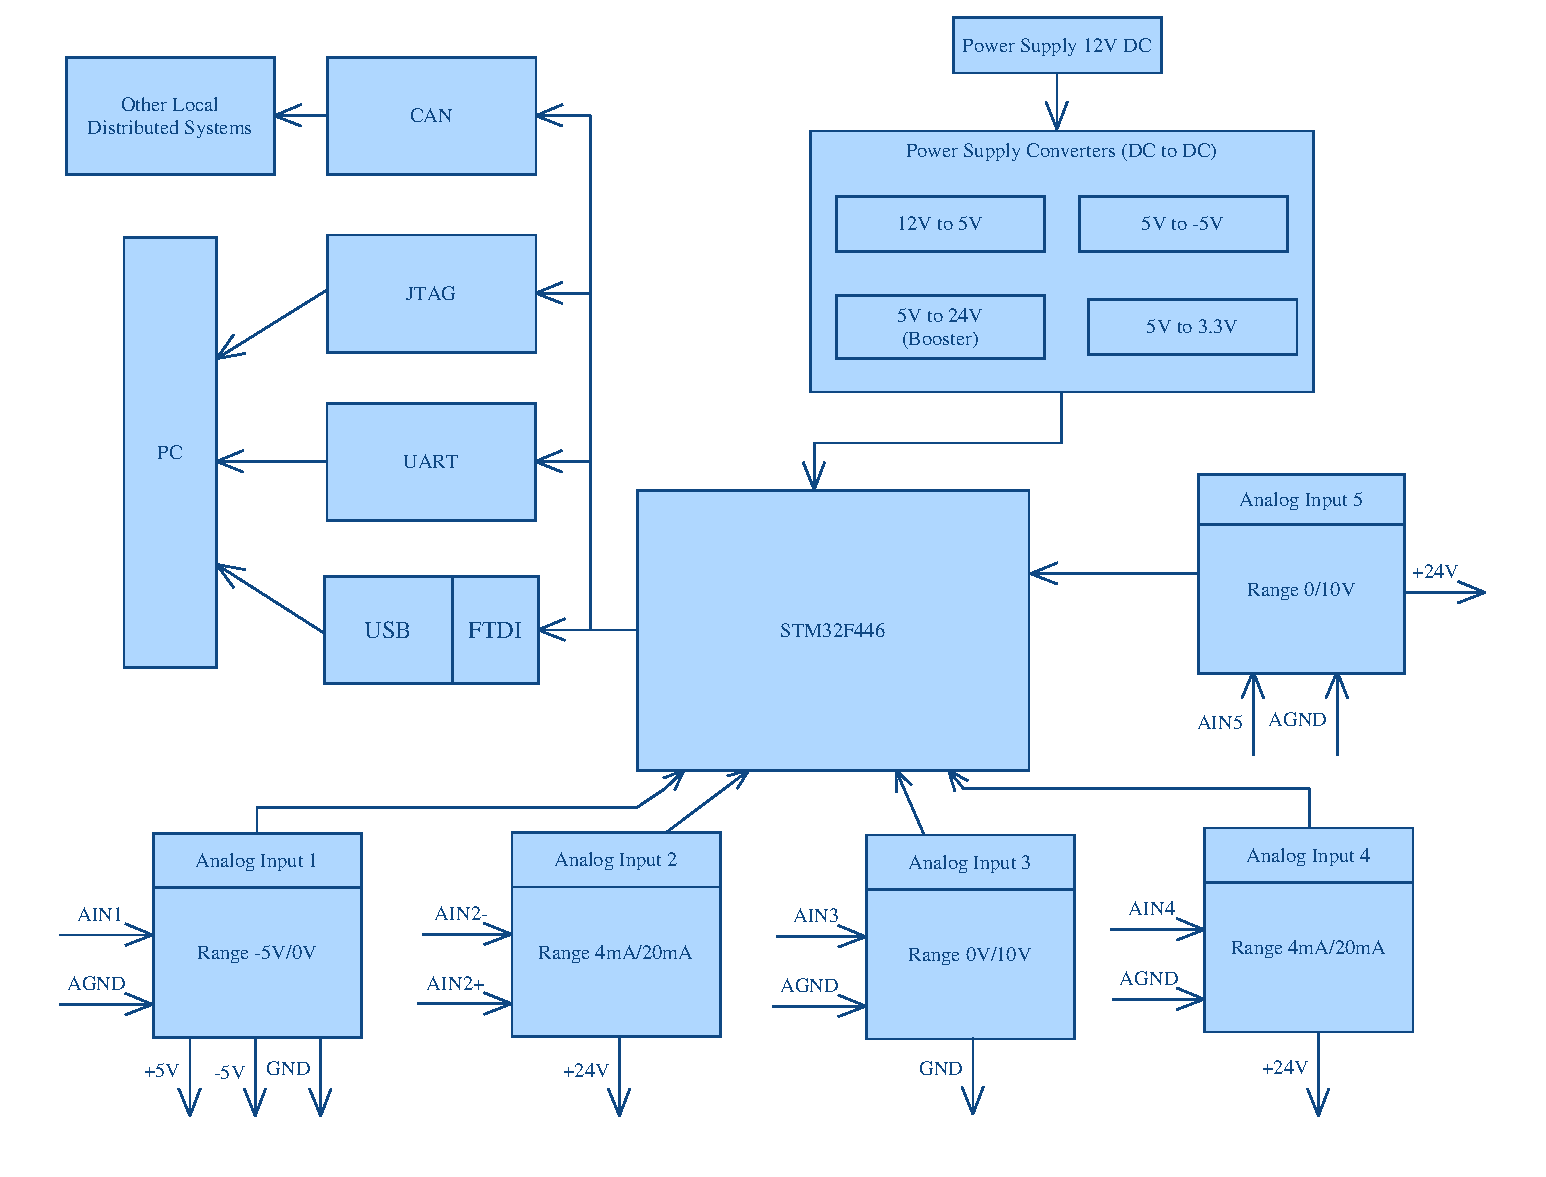
\includegraphics[width=1.0\textwidth]{blockSchematic4.eps}
	\caption{Block Diagram of the System}
	\label{fig:blockDiagram_HW}
\end{figure}

\subsubsection{Control Unit}
	The main part of the hardware is ARM microcontroller STM32F446 from STMicroelectronics. Its choice was given by a requirement from Rieter CZ s.r.o with a description that it was chosen for its low cost, sufficient performance and company's good long-term experience with manufacturer's support. 
	
	Microcontroller STM32F446 is based on ARM Cortex-M4 technology with ARMv7 architecture \ref{sec:ARM_M3}. With DSP instructions it is capable of handling DSP algorithms such as FFT calculation in very short time (less than $0.5 ms$ for 1024-point FFT). Maximal operation frequency is $180 MHz$ at which gives $225 DMIPS$ (Dhrystone benchmark). The most important features and peripherals of this microcontroller are:
\begin{itemize}
	\setlength{\itemsep}{5pt}
	\item ARM 32-bit Cortex-M4, 180 MHz,
	\item 512 kB of Flash memory,
	\item 128 kB of SRAM,
	\item SWD and JTAG debug interface,
	\item 17 Timers and 3 ADC,
	\item Communication interfaces such as USART, CAN, SPI, SAI, SDIO, I2C, LIN etc.
\end{itemize}	
\subsubsection{Power Supply Converters}
Hardware platform of this system has to provide correct supply voltages to microcontroller and sensors. Supplying the sensors is especially complicated since they require three different voltages:
\begin{itemize}
	\setlength{\itemsep}{5pt}
	\item $5 V$,
	\item $-5 V$,
	\item $24 V$.
\end{itemize}
Voltage supply of the microcontroller is $3.3 V$.

The power supply of the hardware board was required to be $12 V$. Therefore, four DC-DC converters has to be designed, specifically:
\begin{itemize}
	\setlength{\itemsep}{5pt}
	\item $12 V$ to $5 V$,
	\item $5 V$ to $-5 V$,
	\item $5 V$ to $24 V$,
	\item $5 V$ to $3.3 V$.
\end{itemize}

For the first conversion from $12 V$ to $5 V$ was used an integrated step-down voltage regulator LM2594. To obtain $-5 V$ a charge pump inverter TPS60400 was used. The conversion from $5 V$ to $3.3 V$ is done by simple linear regulator MCP1825. The only step-up was necessary to get $24 V$ from $5 V$, for this purpose was chosen step-up voltage regulator LM1577.

Concrete circuits schematics of these converters are added as attachment to the CD annexed with this thesis.

\subsubsection{Sensors and Input Modules}



\section{Algorithm for Sliver Quality Analysis}
Algorithm overview diagram is shown in Fig. \ref{fig:software_overview}. This is simplified representation of software used for sliver quality analysis in microcontroller. The input of the system is a sample - measured by ADC - which represents diameter of the sliver. Required output shall be a variance-length curve which is composed by CV(\%) values calculated for several wavelengths\footnote{\label{footnote1:textileTerms}For explanation of the terms used in this paragraph see chapter XXX}. Each software components are individually described in following paragraphs.

The main principle of designed quality analysis lies in determining the coefficient of variation (CV(\%)) value. This value can be obtain from signal that corresponds to appropriate wavelength (cut length). Different wavelengths can be yielded by filtrating the input signal with lowpass filter that passes only frequencies that correspond to given wavelength. Specifically if it is chosen that signal of wavelengths between $\lambda_{min}$ and $\lambda_{max}$ is required, then signal can contain the frequencies only up to $f_{max}$. Where relation between $\lambda_{min}$ and $f_{max}$ is based on knowledge of the \textit{sliver speed} $v_{s}$\footnote{Speed of winding up sliver during the process of combing.} determined as follows in equation \ref{eq:wavelengthToFreq}:

\begin{equation} \label{eq:wavelengthToFreq}
f_{max} = \frac{v_{s}}{\lambda_{min}}.
\end{equation}

From this, we can see that the lower boundary $\lambda_{min}$ is more important and as matter of notation it is used to specify the whole wavelength range. This means that when speaking of CV(\%) for wavelength of $\lambda$ it is actually meant $\lambda_{min}$.

When sufficient amount of CV(\%) values for different wavelength is obtained, then they are joined in \textit{variance-length curve} (see chapter XXX). This curve can be easily represented graphically and as such it allows users to see quality of sliver for different wavelengths just by looking at the shape of the curve. Taking new samples may cause change in appropriate CV(\%) values, therefore, the variance-length curve is periodically updated. It is important to mention that part of curve with lowest wavelength can be updated several times before even one update of higher wavelengths can be calculated. This is due to the fact that higher wavelengths require significantly more input samples.

\begin{figure}[h]
	\centering
	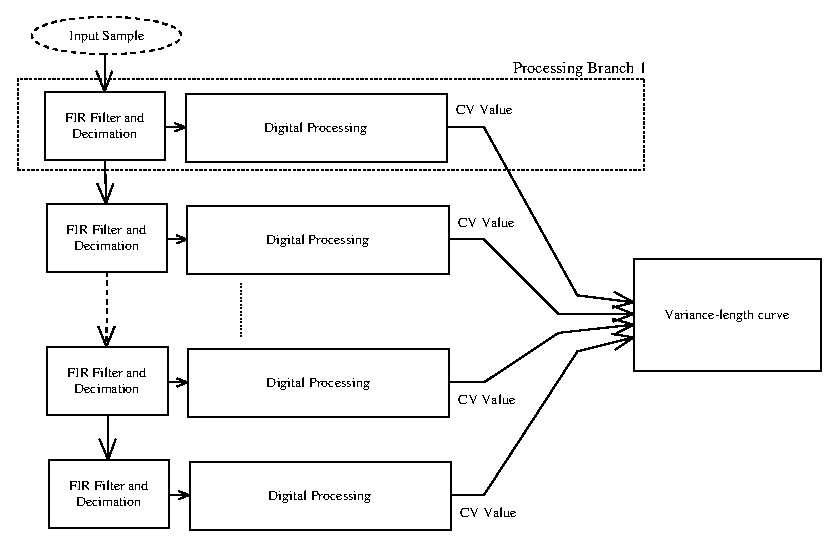
\includegraphics[width=1.0\textwidth]{system_overview.eps}
	\caption{Software Architecture Overview}
	\label{fig:software_overview}
\end{figure}

\subsection{Solution for Embedded Systems Constraints}
\label{sec:SolutionForEmbedded}
As described in chapter \ref{R-T constrains} using embedded systems brings several important constrains. The most significant issues this system has to solve were DSP performance and memory restriction of used microcontroller. The memory issue turned to be critical, because if we had control unit capable of storing hundreds of thousands 16bit samples, we could easily store enough of input samples that allow calculation of all chosen wavelengths and then sequentially use low pass filter to obtain corresponding CV(\%) values. 

This could be done with computer and was used in first version algorithm programmed in MATLAB. However porting software to microcontroller requires usage of decimation (see chapter XXX) which allows us to the lower number of samples used for each stage by throwing out every M-th sample (M is called the decimation factor). Of course, to prevent an \textit{aliasing}\footnote{Effect of violating the Nyqist-Shannon theorem.} low pass filter has to be used to filter out frequencies higher than \textit{Nyquist frequency}\footnote{Half of the sampling frequency}. But, as mentioned in previous paragraphs our application requires use of low pass filter which will always filter out frequencies higher than Nyquist frequency. Thus, no other filter is required prior decimation.

Another issue is limitation of microcontroller is that DSP function for calculation of radix-4 FFT: \textit{cr4\_fft\_1024\_stm32} requires maximally 1024 samples as input. This disallows usage of FFT on much larger amount of samples and processing its frequency spectrum in a way that would also provided us information on the quality of sliver, since (with enough samples) all required frequencies - corresponding to wavelengths - would be visible. This issue is also resolved by decimation of the signal and using multi-rate analysis. 

Using this solution we will only need buffers for 1024 samples, specifically one for each stage of calculation.

\subsection{Wavelengths Specification}
One of the requirements for the software was determined that the device has to be capable of evaluate quality of sliver for wavelengths in range from $0.25 cm$ to $512 cm$ because others wavelengths are not significant enough to the final product. This range is then divided among twelve values, each wavelength representing one stage of calculation. This division will yield each wavelength to be the double of the previous and that allows us to set the decimation factor (see \ref{sec:SolutionForEmbedded}) to $M=2$ for decimators in all stages. The table XXX shows these wavelengths and their corresponding sampling frequencies $f_s$ calculated according to equation \ref{eq:wavelengthToFreq} with sliver speed $v_{s}=30 cm/s$. 

This sliver speed was chosen as it is default settings of combing machines and was used during testing. If different sliver speed is set on combing machine, its value is send over a CAN communication during initialization and basic sampling frequency is adjusted in a way that decimation factor always stays set on $M=2$. This allows to use the same filter coefficients independently on set sliver speeds.

Knowing these informations allows us to determine a \textit{cut off frequency}\footnote{XXX} $f_c$ of FIR filters that are used for limiting the bandwidth and an anti-aliasing. This is done according to the formula $f_c=f_s/2$ for each wavelength as shown in table XXX.

\begin{table}[htbp]
	\centering
	\caption{Wavelengths and corresponding frequencies}
	\begin{tabular}{crrrrr}
		\toprule
		Index of Stage & $\lambda_{min} [cm]$ & $\lambda_{max} [cm]$ & $\lambda_{s} [cm]$ & $f_s [Hz]$ & $f_c [Hz]$ \\
		\midrule
    1     & 0,25  & 0,5   & 0,125 & 240   & 120 \\
    2     & 0,5   & 1     & 0,25  & 120   & 60 \\
    3     & 1     & 2     & 0,5   & 60    & 30 \\
    4     & 2     & 4     & 1     & 30    & 15 \\
    5     & 4     & 8     & 2     & 15    & 7,5 \\
    6     & 8     & 16    & 4     & 7,5   & 3,75 \\
    7     & 16    & 32    & 8     & 3,75  & 1,875 \\
    8     & 32    & 64    & 16    & 1,875 & 0,9375 \\
    9     & 64    & 128   & 32    & 0,9375 & 0,46875 \\
    10    & 128   & 256   & 64    & 0,46875 & 0,234375 \\
    11    & 256   & 512   & 128   & 0,234375 & 0,1171875 \\
    12    & 512   & 1024  & 256   & 0,1171875 & 0,05859375 \\

		\bottomrule
	\end{tabular}%
	\label{tab:Wavelengths}%
\end{table}%


\subsection{Flowchart Diagram}
\section{Description of Designed System}
\subsection{Block Diagram}
\section{Implementation of Software}
\subsection{Filtration}
%For practical spectral analysis like this, we deal with finite duration discrete-time signals, whose spectrum is given by the DTFT. The N-point FFT is merely used to evaluate samples of the DTFT at N equally spaced frequencies omega=2pik/N, 0 leq n leq N-1. Therefore we needed to use good window (like Hann) and oversample DTFT.
\subsection{Detection of Defects}
\subsection{Automatic Evaulation}
\subsection{Example of Designed Application}
\section{Implementation of Hardware}
\subsection{Electronic Circuits Design}
\subsection{Description of possible sensors}
\subsection{Designed Prototype}
\chapter{Conclusions}


\medskip

\begin{proof}\begin{enumerate} \item[8] Bla \item Blo \end{enumerate} \end{proof}

\appendix

\printindex

\appendix

%\bibliographystyle{amsalpha}
\bibliographystyle{siam}
\bibliography{ctuDIP_biblio}

\ctutemplate{specification.as.chapter}

\end{document}